\chapter{Data analysis for gravitational waves}\label{DA}

The quest for detection of weak gravitational wave signals produced by CBCs has required technological improvements in the instruments, and the usage of optimal filtering techinques. Different approaches have used either time domain or frequency domain representations of data and waveform models to take advantage of the currently available computing power and numerical methods.

Fortunately, the extraction of such waves from noisy data can be translated into a well-posed mathematical problem: filter out a signal of known/partially-known shape from a noise-dominated set of samples \cite{Maggiore:2007ulw, Creighton:2011zz, Sathyaprakash:2009xs}. The theory of linear filters has been used to attack such a problem ever since the existence of radar\cite{Wainstein:1962vrq} and has a complete mathematical infrastructure that can be used to search for signals buried in noise and further estimate their parameters using the bayesian statistics framework.



\section{Signal processing:time series and the frequency domain}

Gravitational wave strain data from ground-based L-shaped detectors is currently provided by the LVK collaboration through the GWOSC portal and is made publicly available a few months after each observing run ends \cite[section-3]{LIGOScientific:2019lzm}. This data is obtained from the L-shaped interferometers where the readout of a photodiode sampled in time either at 4 or 16 kHz.


%is translated into equivalent armlength changes or variations in the proper distances between the test masses denoted as strain, i.e., $\delta l/L$, and sampled in time either at 4 or 16kHz. 

To search for CBC signals, existing search pipelines like PyCBC \cite{Usman:2015kfa}, GstLAL\cite{Sachdev:2019vvd}, or MBTA\cite{Aubin:2020goo} use different filtering algorithms, that employ the signal representation either in the time domain, or frequency domain. The Fourier, Laplace, and the Z-transformations allow to go back and forth between both domains. However, in contrast to the other two, the Fourier transform is given by a simpler bijective mapping:

\begin{equation}
\label{eq:1}
X(f) = \int_{-\infty}^{+\infty} x(t)\cdot e^{-i2\pi f t} dt
\end{equation}

\begin{equation}
\label{eq:2}
x(t) = \int_{-\infty}^{+\infty} X(f)\cdot e^{+i2\pi f t} df
\end{equation}

Equations \ref{eq:1} and \ref{eq:2} are used in numerous real-life applications of signal processing and reveal much more information than its time series representation alone. Both representations complement each other and can have different advantages depending on what one is looking for in the data. 

The frequency domain representation can tell us about:

\begin{itemize}
\item 
The frequency content present in a signal. It can be obtained from equation \ref{eq:1}, and extracted from its amplitude spectrum $|X(f)|$.
\item 
The phase of each frequency component. It can be computed by using 

\begin{equation}
\angle X(f) = \arctan\left[\frac{Im\{X(f)\}}{Re\{X(f)\}}\right]
\end{equation}

\end{itemize}

While its timeseries representation makes it easier to read signal features like:

\begin{itemize}
\item Time evolution of the data.
\item Seasonal changes.
\item Linear or quadratic drifts in the data.
\item Shape patterns related to amplitude or phase modulation.

\end{itemize}

The following figure respresents the function 

\begin{equation}\label{tS}
x(t) = \cos(2\pi t) + cos(2\pi\cdot 5\cdot t + \frac{\pi}{4}) + cos(2\pi\cdot 9\cdot t),
\end{equation}

and its used to depict how a the information of a signal that looks complicated, may be extracted by using the Fourier transform.

\begin{figure}[hbt!]
\begin{center}
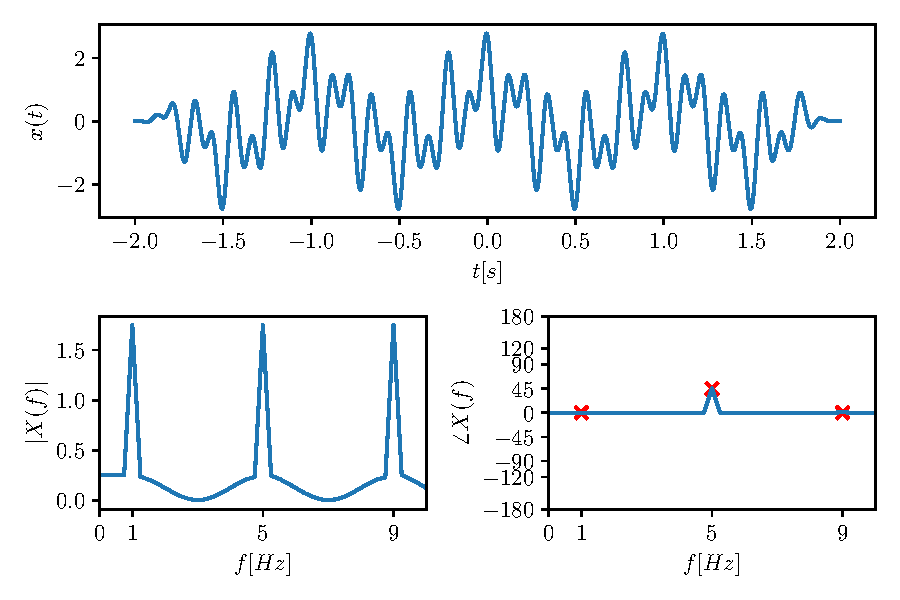
\includegraphics[width=0.6\textwidth, angle=0]{images/Data_analysis/sig_proc/2_1.pdf}
\captionsetup{width=0.8\textwidth}
\caption{Spectral analysis of a "complicated" time-series.}
\caption*{This figure shows a time-domain representation of equation \ref{tS}(top). Its amplitude spectrum(lower left) and phase spectrum(lower right) help unveil the signal content. Notice that the signal in the upper panel has been multiplied by a tukey window with parameter 0.1 to avoid spectral leakage.}
\label{fig:1}
\end{center}
\end{figure}

\FloatBarrier

%A simple example is shown in figure \ref{fig:1}, where what looks very complicated in the time domain can be easily read off in the frequency domain from the magnitude and phase of the complex-valued transformed version of the data: A sum of 3 cosine functions with frequencies 1, 5 and 9 Hz and phases 0, $\frac{\pi}{4}$ and 0 radians respectively.


Some other techniques like spectrograms, and the Q-transform used by the LVK collaboration \cite{LIGOScientific:2017vwq} have been widely used to highlight the frequency content and evolution of a signal and rely on Fourier transforms at their core. The following picture serves as an example of how a BNS GW signal can be represented in the time-frequency plane to identify the power of its frequency components throughout its whole evolution.


\begin{figure}[hbt!]
\begin{center}
\begin{tabular}{cc}
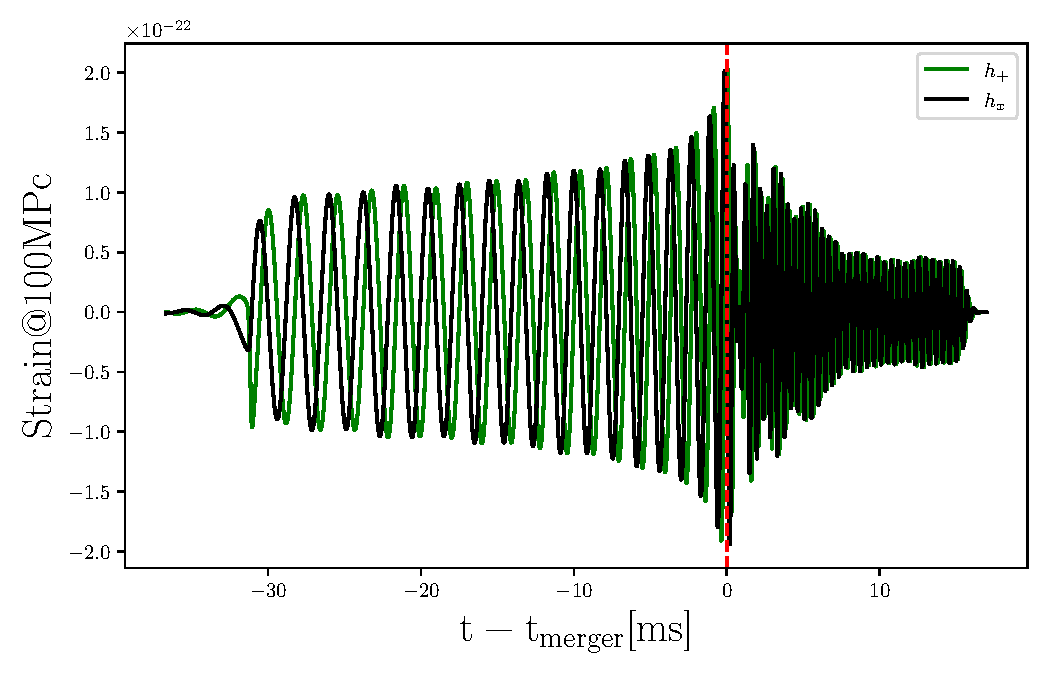
\includegraphics[width=0.45\textwidth, angle=0]{images/Data_analysis/sig_proc/2_2L.pdf}

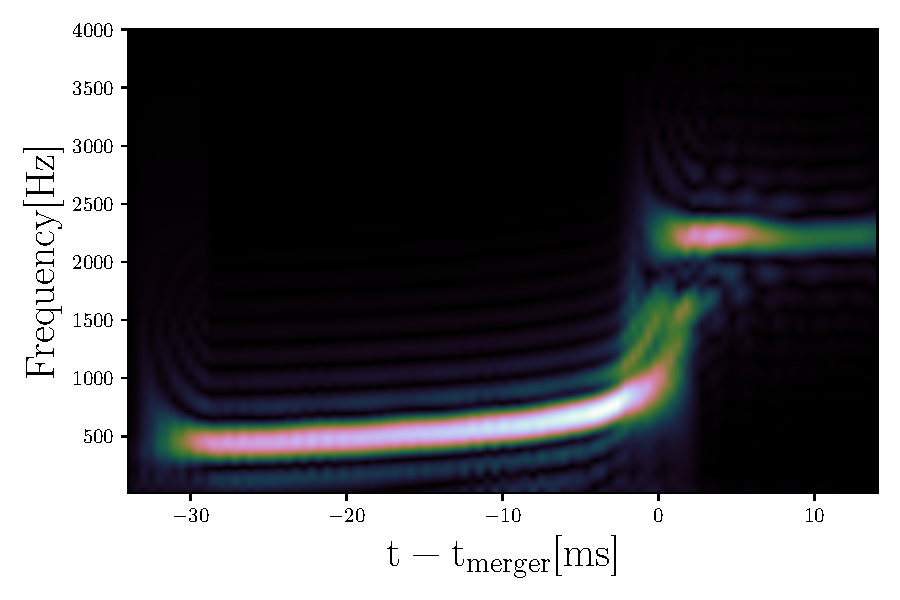
\includegraphics[width=0.45\textwidth, angle=0]{images/Data_analysis/sig_proc/2_2R.pdf}
\end{tabular}
\end{center}
\captionsetup{width=0.8\textwidth}
\caption{Time-frequency representation of a BNS waveform.}
\caption*{This figure represents a BNS waveform taken from the CoRe BNS catalog \cite{Dietrich:2018phi}. It stablishes a parallelism between what one can read from its time-domain representation(left) and the additional information that can be extracted from a spectrogram(right).}
\label{fig:2}
\end{figure}

\FloatBarrier

In the context of gravitational-wave astronomy, such a simple bijection mapping between both domains has been widely used. Depending on the problem, some modelled and unmodelled search algorithms, as well as waveform models rely on either one representation or the other to improve computational performance. However, the simplicity of Fourier transforms gives much flexibility to go back and forth the time and frequency domain while developping filtering algorithms. 


\section{Convolution and cross-correlation}

The problem of waveform extraction from a noisy datastream can be mathematically defined using the integral equation for an optimal filter(see Wainstein \cite[chapter X]{Wainstein:1962vrq}). Such procedure and can lead to different optimal linear filters depending on the kind of problem one wants to solve. 

This section uses convolutions and cross-correlations to motivate the idea of filtering techniques from the perspective of \textit{sliding inner products}. It makes a lot of sense trying to find a mathematical operator that takes two signals and returns a number that accounts for how similar or "correlated" they are. More rigorously, such filter operations can be treated as inner products in an infinite dimensional vector space, which gives the problem a more geometric fashion, i.e. "a manifold of waveforms equipped with a metric" \cite{Andersson:2019yve,Creighton:2011zz}.

let $\mathcal{F}$ be the set of all complex-valued functions, we can define both operations as bilinear maps from $\mathcal{F}\times\mathcal{F}$ to $\mathcal{F}$:

\vspace{1cm}

\begin{center}

\begin{tabular}{cccc}
$conv_\tau:$&$\mathcal{F}\times\mathcal{F}$ & $\rightarrow$ & $\mathcal{F}$ \\
&$(h, q)$ &$\mapsto$ & $conv(h,q)(\tau)$
\end{tabular}

\end{center}

\vspace{1cm}

\begin{center}

\begin{tabular}{cccc}
$corr_\tau:$&$\mathcal{F}\times\mathcal{F}$ & $\rightarrow$ & $\mathcal{F}$ \\
&$(h, q)$ &$\mapsto$ & $corr(h,q)(\tau)$
\end{tabular}

\end{center}

\vspace{1cm}

Both operators, can either be represented easily in the time domain and frequency domain. In the time domain, they take the form of integral operators 

\begin{equation}\label{eq:3}
conv(h, q)(\tau)= \int_{-\infty}^{\infty} h(t)q(t-\tau)dt
\end{equation}


\begin{equation}\label{eq:4}
corr(h, q)(\tau)= \int_{-\infty}^{\infty} h^*(t)q(t+\tau)dt
\end{equation}

To see how operators \ref{eq:3} and \ref{eq:4} act as \textit{sliding inner products} we will use discrete finite square waves $\vec{h}$, $\vec{q}$, and the operator \ref{eq:3} in its discrete form 


\vspace{0.5cm}

\begin{center}

\begin{tabular}{c}
$ \vec{q} = [0,1,1,0,0,0]$ \\
$ \vec{h} = [0,0,1,1,0,0]$

\end{tabular}

\end{center}

\vspace{0.5cm}

\begin{equation}\label{eq:7}
corr_{\tau} = \sum_{n=\infty}^{\infty} (h^*_{n} \cdot q_{n+\tau}) \cdot \Delta t
\end{equation}


Where $h_i$ and $q_j$  are the values of $\vec{h}$, $\vec{q}$ along the time axis. One can read $corr_\tau$ as the components of a finite array where each component represents  the result of a 3-step operation between $\vec{q^*}$ and $\vec{h}$:

\begin{enumerate}
\item A slide(shift) of $\vec{q^*}$ in the time axis.
\item A slot wise multiplication.
\item A sum of all $\tau$ components
\end{enumerate}

To see this explicitly, lets use different values of $\tau$, and expand the summation \ref{eq:7} 

\begin{itemize}

\item For $\tau = -4$, expanding the sum in equation \ref{eq:5}, and using $\Delta t = 1$, looks like:

\begin{multline}
corr_{-4} = ...+h^{*}_{0}\cdot q_{0-4}+ h^{*}_{1}\cdot q_{1-4} + h^{*}_{2}\cdot q_{2-4}+ \\h^{*}_{3}\cdot q_{3-4} + h^{*}_{4}\cdot q_{4-4} + h^{*}_{5}\cdot q_{5-4} + h^{*}_{6}\cdot q_{6-4}+...
\end{multline}

\begin{multline}
corr_{-4} = ...+h^{*}_{0}\cdot q_{4}+ h^{*}_{1}\cdot q_{-3} + h^{*}_{2}\cdot q_{-2} +\\ h^{*}_{3}\cdot q_{-1} + h^{*}_{4}\cdot q_{0} + h^{*}_{5}\cdot q_{1} + h^{*}_{6}\cdot q_{2}+... = 0
\end{multline}


\begin{center}

\begin{tabular}{c|c|c|c|c| c|c|c|c|c|c |c|c|c|c|}

$\vec{q} \rightarrow$&0&1&1&0&0&0 &\textcolor{red}{0}&\textcolor{red}{0}&\textcolor{red}{0}&\textcolor{red}{0}&\textcolor{red}{0}&\textcolor{red}{0}&\textcolor{red}{0}&\textcolor{red}{0}\\

\hline
$\vec{h} \rightarrow$&\textcolor{red}{0}&\textcolor{red}{0}&\textcolor{red}{0}&\textcolor{red}{0}&0&0&1&1&0&0&\textcolor{red}{0}&\textcolor{red}{0}&\textcolor{red}{0}&\textcolor{red}{0}
\end{tabular}

\end{center}


\item For $\tau = 0$, $corr_{0}=1$

\begin{center}

\begin{tabular}{c |c|c|c|c| c|c|c|c|c|c |c|c|c|c|}
$\vec{q} \rightarrow$&\textcolor{red}{0}&\textcolor{red}{0}&\textcolor{red}{0}&\textcolor{red}{0}
&0&1&1&0&0&0&\textcolor{red}{0}&\textcolor{red}{0}&\textcolor{red}{0}&\textcolor{red}{0}\\
\hline
$\vec{h} \rightarrow$&\textcolor{red}{0}&\textcolor{red}{0}&\textcolor{red}{0}&\textcolor{red}{0}&0&0&1&1&0&0&\textcolor{red}{0}&\textcolor{red}{0}&\textcolor{red}{0}&\textcolor{red}{0}
\end{tabular}

\end{center}


\item For $\tau = +4$, $corr_{+4}=0$

\begin{center}

\begin{tabular}{c|c|c|c|c| c|c|c|c|c|c |c|c|c|c|}

$\vec{q} \rightarrow$&\textcolor{red}{0}&\textcolor{red}{0}&\textcolor{red}{0}&\textcolor{red}{0}&\textcolor{red}{0}&\textcolor{red}{0}&\textcolor{red}{0}&\textcolor{red}{0}&0&1&1&0&0&0\\

\hline
$\vec{h} \rightarrow$&\textcolor{red}{0}&\textcolor{red}{0}&\textcolor{red}{0}&\textcolor{red}{0}&0&0&1&1&0&0&\textcolor{red}{0}&\textcolor{red}{0}&\textcolor{red}{0}&\textcolor{red}{0}
\end{tabular}

\end{center}

\end{itemize}

\vspace{1cm}

Using a few more samples can help visualize the result of the inner product as a function of timeshift, e.g. taking just the samples [-5, 5], the result for the correlation is:

$$corr_\tau = [...,0,0,0,0,0,1,2,1,0,0,0 ,...]$$



\begin{figure}[hbt!]
\begin{center}
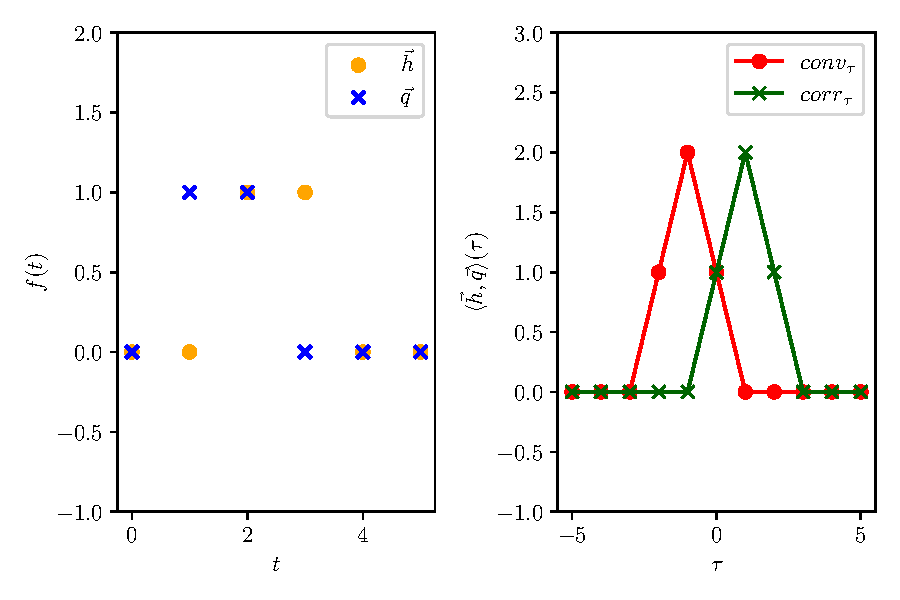
\includegraphics[width=0.8\textwidth, angle=0]{images/Data_analysis/sig_proc/corr.pdf}
\captionsetup{width=0.8\textwidth}
\caption{Discrete cross-correlation of two box-pulses}
\caption*{Time domain representation of 2 timeshifted boxcar pulses(left) and the results of their convolution and cross-correlation(right). Notice that both operations are each other's time reversal.}
\label{fig:3}
\end{center}
\end{figure}

\FloatBarrier


Nevertheless, most modern software executes this operations using the frequency domain representation of equations \ref{eq:3} and \ref{eq:4} which looks much simpler

\begin{equation}\label{eq:5}
F \left(conv(h,q)(\tau) \right)= \left( h(f) \cdot q(f) \right)(\tau)
\end{equation}


\begin{equation}\label{eq:6}
F \left( corr(h,q)(\tau) \right)= \left( h(f) \cdot q^*(f) \right) (\tau)
\end{equation}




\newpage

\section{Matched filtering}

In contrast to the ideal scenario shown in figure \ref{fig:2} where the signal can be resolved perfectly, the signals detected so far by the LVK collaboration \cite{LIGOScientific:2021djp} are buried in instrumental noise. The sprectrograms computed for interferometer data around events of astrophysical origin look as follows 

\begin{figure}[hbt!]
\begin{center}
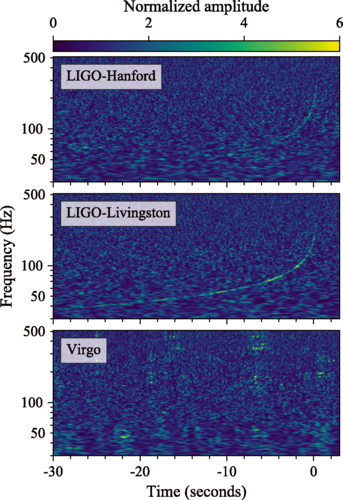
\includegraphics[width=0.5\textwidth, angle=0]{images/170817mult.png}
\captionsetup{width=0.8\textwidth}
\caption{Multidetector detection of GW170817 without glitch.}
\caption*{This image was taken from \cite{LIGOScientific:2017vwq}. It shows the sprectrogram computed around the GW170817 event for LIGO-Virgo detector network.}
\label{ofeijf}
\end{center}

\end{figure}

To reach highest sensitivity GW astronomers use a modelled search algorithm called \textit{matched filtering}. Such algorithm uses prior knowledge about the signal and detector sensitivity estimates to focus particularly on the following problem:

"Extracting a signal of known morpholohy, burried in frequency-dependent Gaussian noise of known power spectral density(PSD)"

However, its important to remark that the matched filtering algorithm can become computationally expensive. For this reason, other suboptimal unmodelled filtering techniques are used for low latency searches, such as cWB and Bayeswave \cite{Drago:2020kic, Cornish:2014kda}. In addition, in some cases detector data can have non-gaussian transients called "glitches", that can mask signals of astrophysical origin. The follwing figure shows illustrates the impacts of a glitch appearing in LIGO livingston data during the event GW170817
 

\begin{figure}[hbt!]
\begin{center}
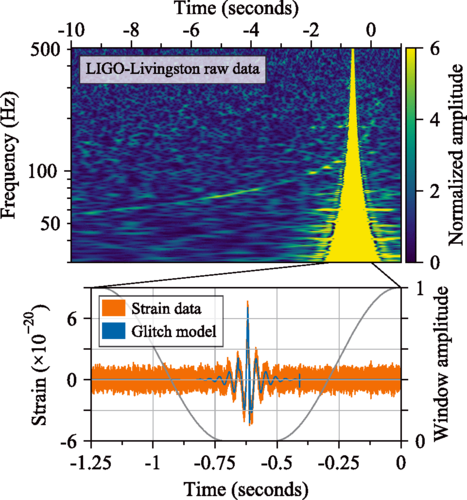
\includegraphics[width=0.5\textwidth, angle=0]{images/170817.png}
\captionsetup{width=0.8\textwidth}
\caption{The glitch around GW170817}
\caption*{This image was taken from \cite{LIGOScientific:2017vwq}. It shows the time-series(top) from LIGO Livingston around the event GW170817 and its time-frequency representation(bottom). Notice the glitch masking the high-frequency part of the chirping signature.}
\label{ijenfo}
\end{center}
\end{figure}

\FloatBarrier

The following is going to be a derivation of the matched filtering signal-to-noise ratio(SNR) equation for a single detector, motivated by what is presented in \cite{Sathyaprakash:2009xs,Creighton:2011zz,Maggiore:2007ulw,Saulson:1995zi}. As seen in figures \ref{ofeijf} and \ref{ijenfo} raw interferometric data of ground based detectors is dominated by noise. For that reason, the main problem of gravitational wave astronomy its to decide between follwing two hypotheses:

\begin{itemize}
\item The datastream $h$ is pure instrumental noise
$$ h(t) = n(t)$$
\item The datastream $h$ is a combination of instrumental noise and a signal of astrophysical origin.
$$ h(t) = u(t) + n(t)$$
\end{itemize}


It can be shown that the optimal detection statistic when one looks for signals of known/partially-known morphology in the presence of gaussian stationary noise can be built in terms of the following noise weighted inner products

\begin{equation}\label{eq:8}
\langle h,q \rangle =4 Re\left( \int_{0}^{\infty} \frac{h(f) \cdot q^{*}(f)}{S_n(f)} \cdot df \right)
\end{equation}

Where $h$ is the signal at the detector readout, and $q$ is a theoretical model of a signal from astrophysical origin called \textit{template}. Furthermore, $S_n$ is the one-sided PSD of the detector,  which can be estimated by using an ensemble average via Khinchin's theorem

\begin{equation}\label{PSD}
\langle n(f), n(f') \rangle = \delta(f'-f) \cdot S_n(f)
\end{equation}


Moreover, the phase and arrival time are typically unkown, so we can let the template $q$  include them initially as free parameters. In the frequency domain that can be achieved by adding an additional complex exponential factor 


\begin{equation}
q(f)\rightarrow q\cdot e^{i(2\pi f \tau + \phi_0)}
\end{equation}

The inner product \ref{eq:8} then becomes a function of $\tau$ and $\phi_0$:

\begin{equation}\label{eq:9}
\langle h,q e^{i(2\pi f \tau + \phi_0)} \rangle =4 Re\left( \int_{0}^{\infty} \frac{h(f) \cdot q^{*}(f) }{S_n(f)} \cdot e^{i(2\pi f \tau + \phi_0)} df \right)
\end{equation}

\begin{equation}\label{eq:10}
\langle h,q e^{i(2\pi f \tau + \phi_0)} \rangle =4 Re\left( e^{i \phi_0}\underbrace{\int_{0}^{\infty} \frac{h(f) \cdot q^{*}(f) }{S_n(f)} \cdot e^{i 2\pi f \tau} df}_{Z(\tau)} \right)
\end{equation}


So that we can optimize over the phase by taking the complex magnitude on both sides of the equation \ref{eq:10} and use $\left|e^{i2\pi \phi_0}\right|=1$

\begin{equation}\label{eq:11}
\langle h,q e^{i(2\pi f \tau + \phi_0)} \rangle_{\phi_0=\phi_{opt}} =4 Re\left( \left|e^{i \phi_0}\right|  \left| \int_{0}^{\infty} \frac{h(f) \cdot q^{*}(f) }{S_n(f)} \cdot e^{i 2\pi f \tau} df \right| \right)
\end{equation}

\begin{equation}\label{eq:12}
\langle h,q e^{i(2\pi f \tau + \phi_0)} \rangle_{\phi_0=\phi_{opt}} =4\cdot \left( \left| \int_{0}^{\infty} \frac{h(f) \cdot q^{*}(f) }{S_n(f)} \cdot e^{i 2\pi f \tau} df \right| \right)
\end{equation}

\begin{figure}[hbt!]

\begin{center}

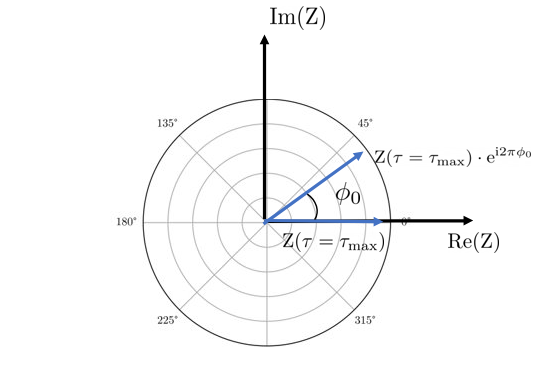
\includegraphics[width=0.4\textwidth, angle=0]{images/ph_opt.png}
\caption{Phase optimization in the complex plane}
\label{fig:6}
\end{center}
\end{figure}

\FloatBarrier

However, it is useful to write equation \ref{eq:12} in terms of double-sided integrals. In such form, the inner product looks like an inverse Fourier transform

\begin{equation}\label{eq:13}
\langle h,q e^{i(2\pi f \tau + \phi_0)} \rangle_{\phi_0=\phi_{opt}} =4\cdot \left( \left| \int_{-\infty}^{\infty} \theta(f)\frac{h(f) \cdot q^{*}(f) }{S_n(|f|)} \cdot e^{i 2\pi f \tau} df \right| \right)
\end{equation}


Writing equation \ref{eq:13} in such form is more convinient in the context of modern filtering algorithms. Modern computers can compute discrete Fourier transforms(DFTs) much faster(using the fast fourier transform algorithm(FFT)) than evaluating the integral \ref{eq:13} iteratively for each $\tau$ value. Notice that $\theta(f)$ is the Heaviside step function given by

\begin{equation}\label{eq:14}
\theta(f) = \begin{cases}
 1 &, f \geq 0 \\
 0 &, f < 0
\end{cases}
\end{equation}

Now, let us write equations \ref{eq:13} of discrete sums and finite increments

$$\int \rightarrow \sum $$
$$ \delta t \rightarrow \Delta t$$ 
$$\delta f \rightarrow \Delta f$$

\begin{equation}
FT(x(t))=\int_{-\infty}^{+\infty} x(t)\cdot e^{-i2\pi f t} dt \rightarrow  FFT(x)\cdot \Delta t = \sum_{j=-\infty}^{+\infty} x_j \cdot e^{-i2\pi f j} \cdot \Delta t
\end{equation}

\begin{equation}
IFT(x(t))=\int_{-\infty}^{+\infty} X(f)\cdot e^{+i2\pi f t} df \rightarrow  IFFT(X)\cdot \Delta f = \sum_{j=-\infty}^{+\infty} X_j \cdot e^{+i2\pi f j} \cdot \Delta f
\end{equation}


\textbf{Remark:} Notice that in realistic applications, time-series require proper sampling $\Delta t$ to avoid aliasing(see Nyquist theorem \cite{5055024}). 

Finally, we arrive at a discrete version of equation \ref{eq:13}, written in terms of IFFTs which will return a complex-valued time series

\begin{equation}\label{eq:15}
\langle \vec{h} ,\vec{q} \cdot e^{i(2\pi j \tau + \phi_0)} \rangle_{\phi_0=\phi_{opt}} =4\cdot \left| \mathrm{IFFT}\left(  \theta \cdot \frac{h \cdot q^{*} }{S_n} \right)\right|(\tau) \cdot \Delta f
\end{equation}


The recovered SNR $\rho(\tau)$, also called "overlap" when optimizing over the phase, is obtained by normalizing $\langle h,q e^{i(2\pi f \tau + \phi_0)} \rangle_{\phi_0=\phi_{opt}}$, using the norm of the template $q$

\begin{equation}
\rho (\tau) = \frac{\langle h,q e^{i(2\pi f \tau + \phi_0)} \rangle_{\phi_0=\phi_{opt}}}{\sqrt{\langle q,q \rangle}}
\end{equation}


\begin{equation}\label{eq:17}
\rho (\tau)= 
\frac{
4\cdot \left| \mathrm{IFFT}\left(  \theta \cdot \frac{h \cdot q^{*} }{S_n}\right)\right| (\tau) \cdot \Delta f
}
{
\sqrt{4\cdot \sum_{-\infty}^{\infty} \frac{q\cdot q^*}{S_n} \Delta f}
}
\end{equation}

It can be shown that the optimal SNR(see \cite[chapter 5]{Sathyaprakash:2009xs}) is given by the inner product of the signal with itself

\begin{equation}
\rho_{opt} = \langle h,h \rangle^{\frac{1}{2}} = \left[4\cdot\int_{0}^{\infty} \frac{h(f)h^{*}(f)}{S_n(f)}df\right]^{\frac{1}{2}}
\end{equation}

\begin{equation}\label{sopt}
\rho_{opt} = \langle h,h \rangle^{\frac{1}{2}} = \left[4\cdot\sum_{0}^{\infty} \frac{ h\cdot h^{*}}{S_n}\Delta f\right]^{\frac{1}{2}}
\end{equation}

Tipycally, waveform modelling studies compare the maximum recovered SNR value of $\rho(\tau=\tau_{max})$ with the optimal SNR $\rho_{opt}$ for a given injected waveform. The following quatities are often used for that matter 


\begin{equation}
M = 1-\frac{\rho(\tau)|_{\tau_{max}}}{\rho_{opt}}
\end{equation}

\begin{equation}
\alpha = \frac{\rho(\tau)|_{\tau_{max}}}{\rho_{opt}} \rightarrow \alpha = 1-M
\end{equation}

Where M is called \textit{mismatch}, and $\alpha$ can be used to talk naturally about SNR recovery percentages. The following figure shows the results obtained from overlapping a BNS postmerger waveform with a finite monochromatic wave. Notice that  the optimal values for $\tau$ and $\phi_0$ are taken at the maximum of SNR envelope(middle panel)


\begin{figure}[hbt!]
\begin{center}
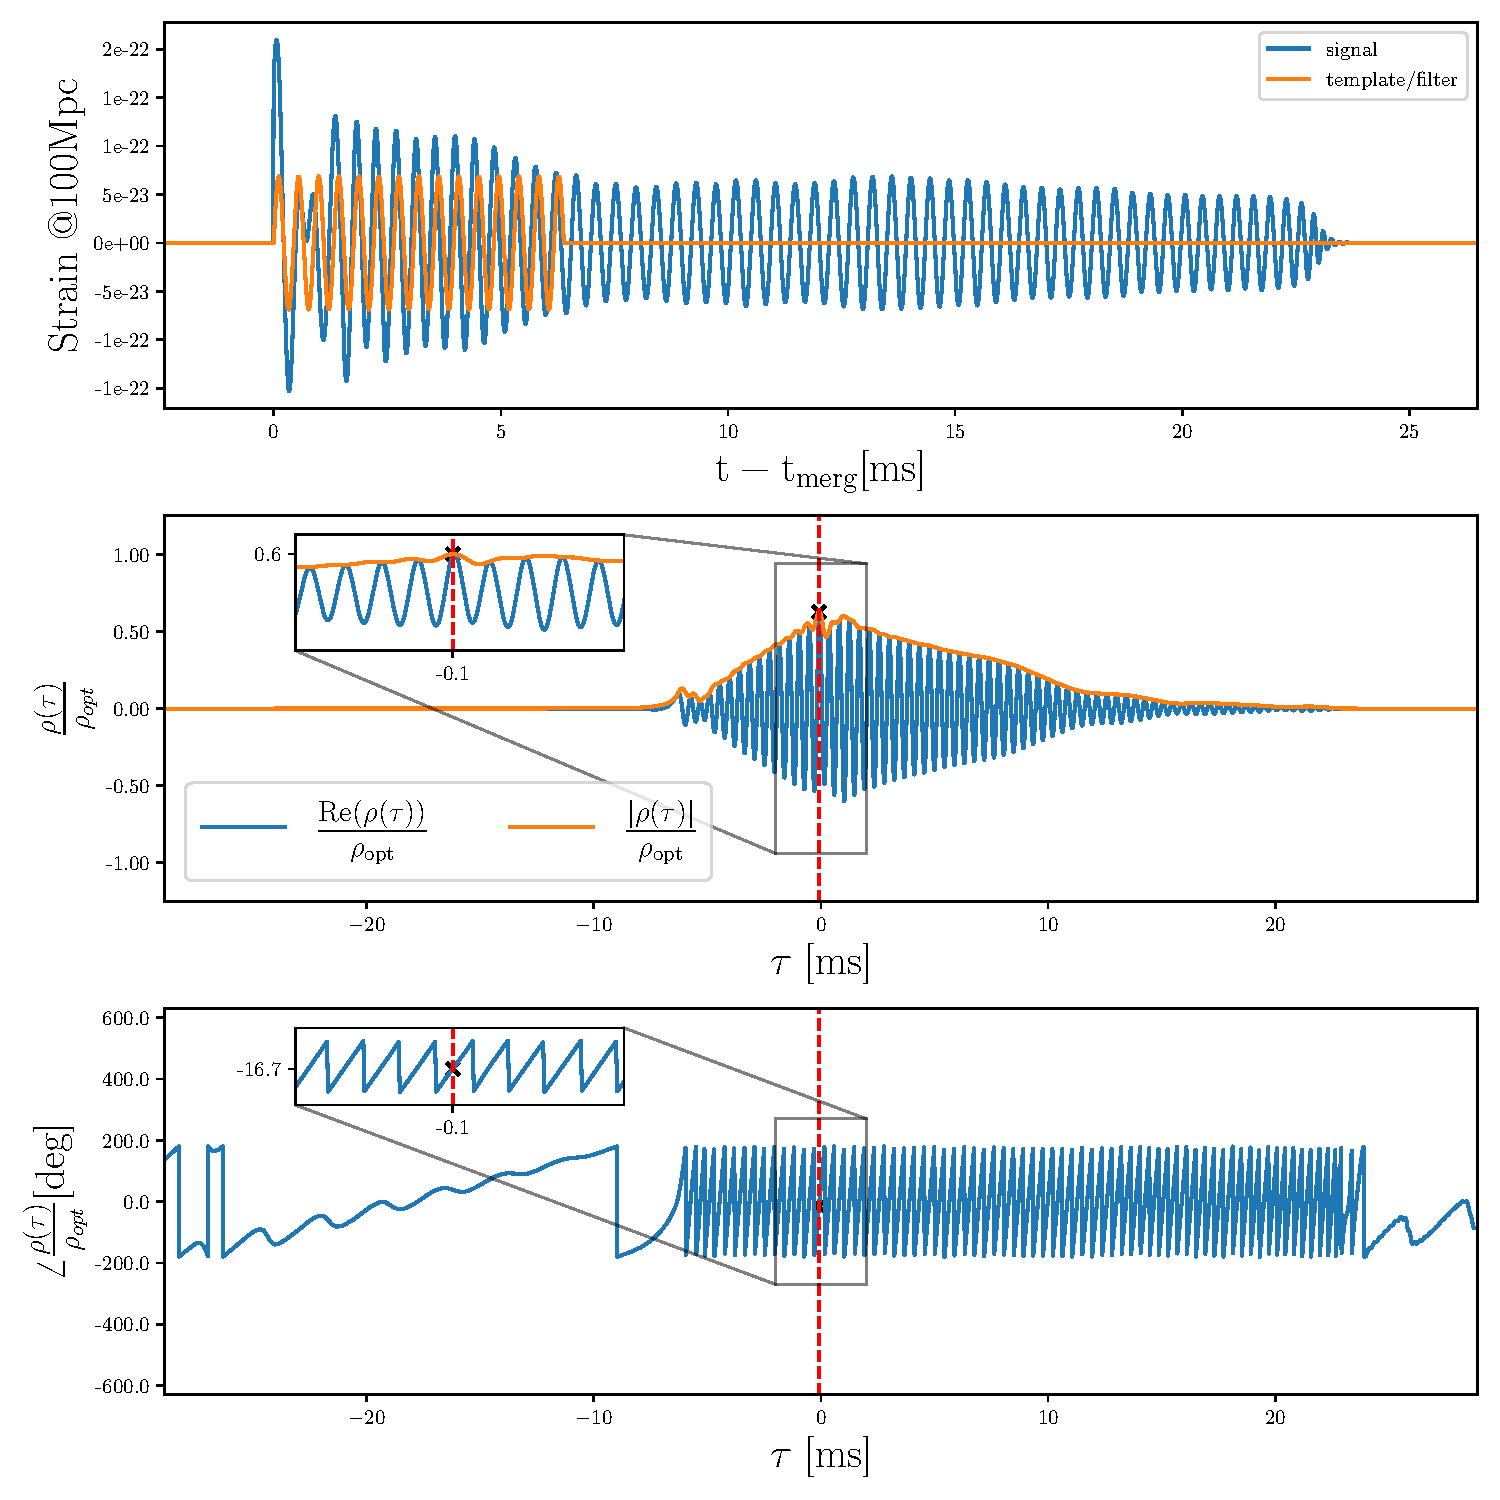
\includegraphics[width=0.8\textwidth, angle=0]{images/Data_analysis/results/ex_search.pdf}
\captionsetup{width=0.8\textwidth}
\caption{From SNR to the optimal timeshift and phaseshift.}
\caption*{This figure shows the overlap of one postmerger GW signal(blue) with a monochromatic template with parameters $\mathrm{f=2270}$ Hz and $\mathrm{d=6.4}$ ms (orange). It depicts how the optimal phase and timeshift is selected.
}
\label{fig:7}
\end{center}
\end{figure}

\FloatBarrier



\section{Ideal vs real inplementation}

Excecuting the matched filtering algorithm to compute the overlap \ref{eq:17} can become extremely tricky and computationally expensive task. The following is a list of technical details that must be taken into account to get consistent results:

\begin{itemize}

\item Signal and template
	\begin{itemize}
	
	\item Signal and template must have the same sampling rate $dt$ and the same length $N$. Most numerical methods for computing DFTs just probe a finite amount of frequency bins, i.e. up to Nyquist frequency. For this reason, the sampling rate and the length of both signals will affect the frequency domain spacing $\mathrm{\Delta f}=\frac{1}{N\cdot dt}$.
	
	\item Zero-padding signals is important. Such technique helps adding enough space for templates to slide against the data, which helps avoiding boundary effects when computing DFTs.
	\item Choosing the right windowing technique helps resolving better signals that have a "rich spectrum". Spectral leakage is something to worry about when computing DFTs. Signals with an amplitude spectrum that have several peaks in neighboring frequency bins will be hard to resolve, unless a tappering window function has been applied to them.
	
	\item The overlap function must be computed for more than one template. Existing waveform models with $n$-free parameters  are known as "template banks". Such generalization turns the inner product \ref{eq:13} into the following n-dimensional object that can become very expensive to compute
	
\begin{equation}\label{inn}
\langle h,q e^{i(2\pi f \tau + \phi_0)} \rangle_{a_1, ..., a_n,\phi_0=\phi_{opt}} =4\cdot \left( \left| \int_{-\infty}^{\infty} \theta(f)\frac{h(f) \cdot q^{*}_{a_1, ..., a_n}(f) }{S_n(|f|)} \cdot e^{i 2\pi f \tau} df \right| \right)(\tau)
\end{equation}

	\end{itemize}
	
\item Power spectral density
	\begin{itemize}
	
	\item In general, current ground based detector design curves are provided with non-uniform sampling rate in the frequency space \cite{Reitze:2019dyk} with cutoffs bewtten 10 Hz and 5 kHz. Because of that, interpolation techniques must be used to define them in the same frequency bins as the data and templates up to Nyquist frequency.
	\item Detector design curves come with a gap between 0 and 10Hz. Since standard FFT methods require to have the zero frequency bin included, one has to figure out a way to fill such gap. This work uses a 2 step approach: computes the inverse PSD between 10 Hz and Nyquist frequency, and then zeropads between [0-10Hz) to avoid dividing by zero in equation \ref{eq:13}.
	\item Standard FFT methods need the negative frequency bins. For that reason, one has to mirror the real-valued PSD to the negative frequency bins.
	\end{itemize}

\end{itemize}

\begin{figure}[hbt!]

\begin{center}

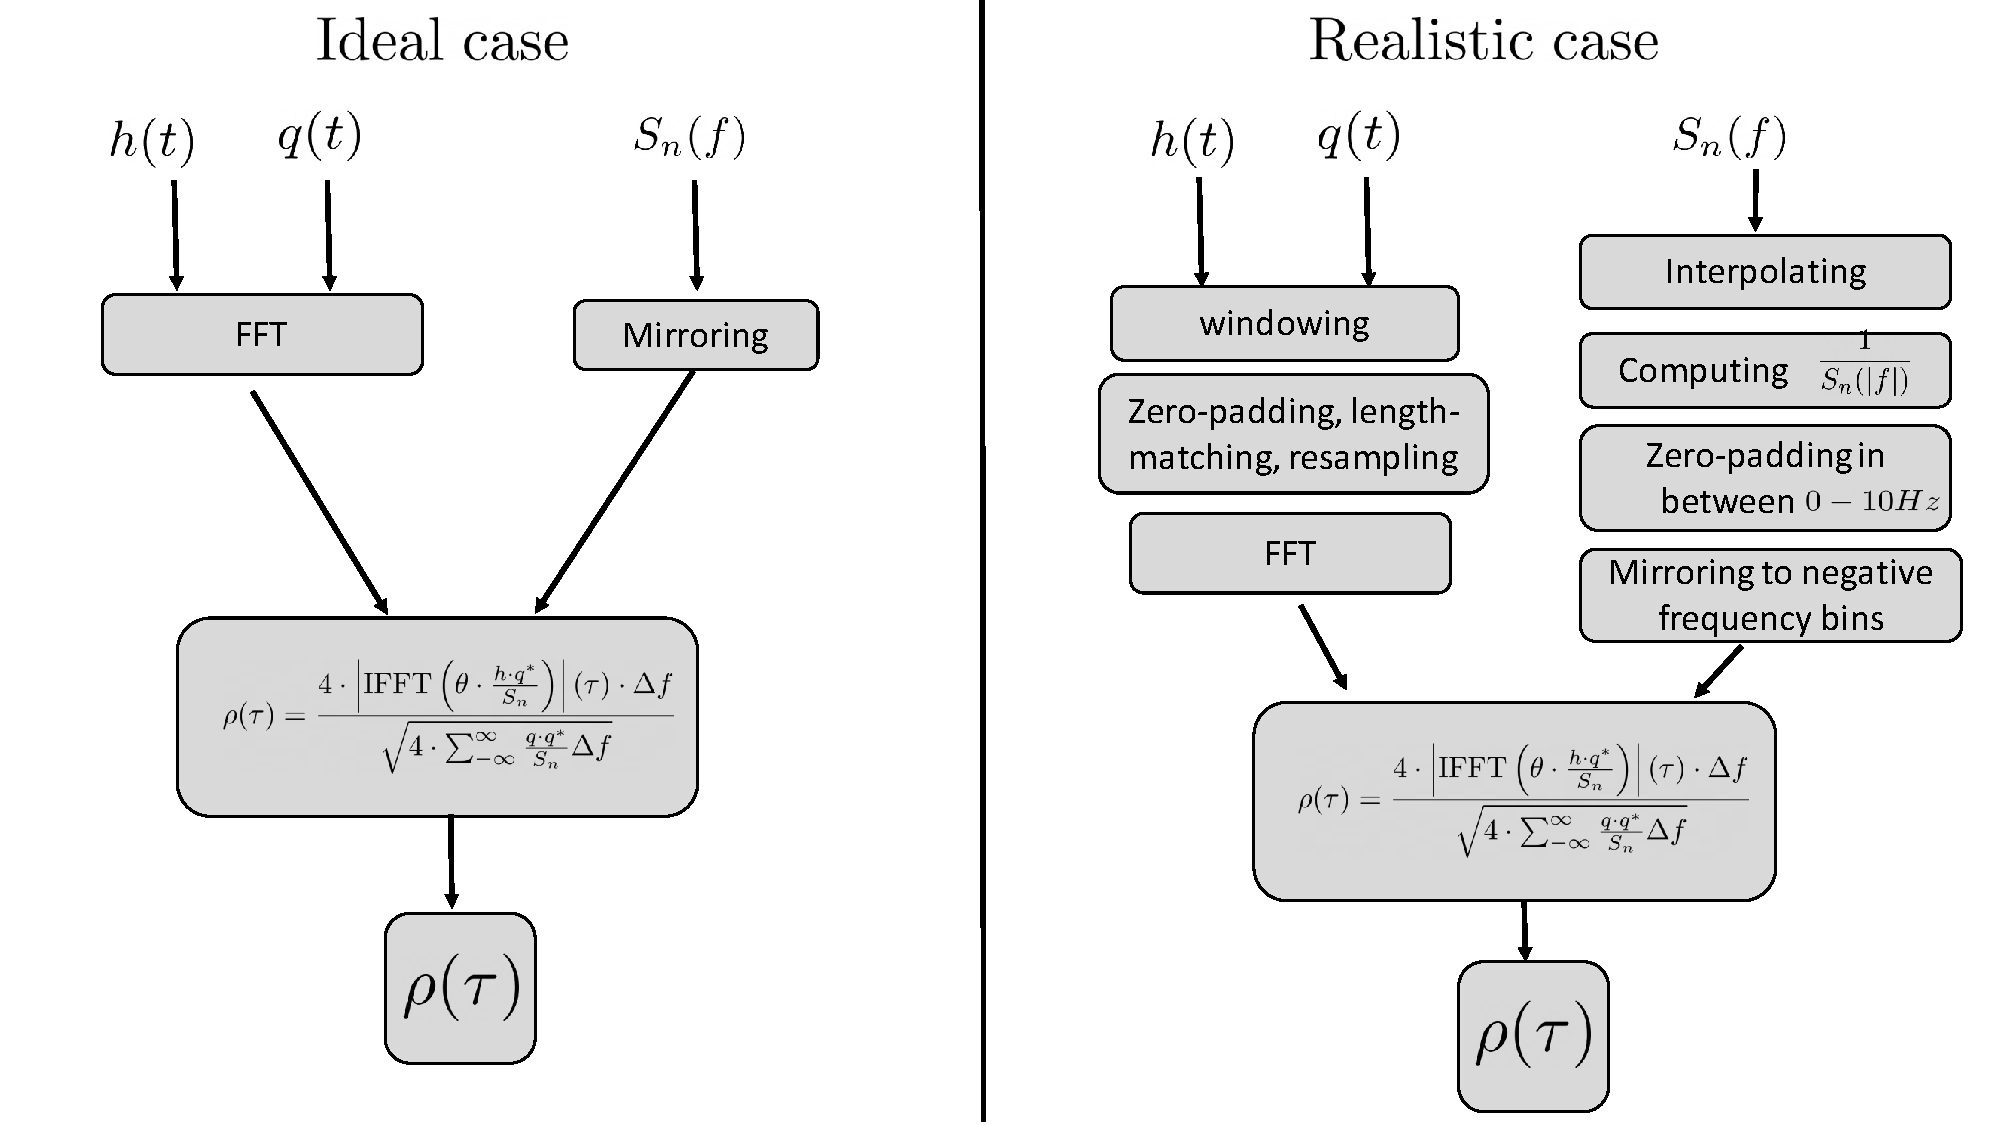
\includegraphics[width=\textwidth, angle=0]{images/comparison.pdf}
\caption{Algorithm implementation comparison flowchart}
\label{fig:8}
\end{center}
This figure establishes a parallel between an ideal implementation of the matched filtering algorithm according to equation \ref{eq:17} (left) and a more realistic implementation considering all technical details(right).
\end{figure}

\FloatBarrier












